\caption{two neighbouring squares}
\label{Figure::filler_square_two}

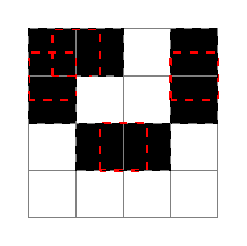
\begin{tikzpicture}[scale=0.3] 
    % Define parameters
    \def\xmin{0}
    \def\xmax{8}
    \def\ymin{0}
    \def\ymax{8}


    \fill[\stepOneColor] (2,2) rectangle (6, 4);
    \fill[\stepOneColor] (6,4) rectangle (8, 8);
    \fill[\stepOneColor] (0,4) rectangle (2, 8);
    \fill[\stepOneColor] (2,6) rectangle (4, 8);
    
    
    \fill[\fillerColor] (3,2) rectangle (5, 4);
    \fill[\fillerColor] (6,5) rectangle (8,7);
    \fill[\fillerColor] (0,5) rectangle (2,7);
    \fill[\fillerColor] (1,6) rectangle (3,8);
    

    \draw[step=2.0,gray,thin] (\xmin,\ymin) grid (\xmax,\ymax);
    
    \draw[dashed,thick, red](3,2) rectangle (5, 4);
    \draw[dashed,thick, red](6,5) rectangle (8, 7);
    \draw[dashed,thick, red](0,5) rectangle (2, 7);
    \draw[dashed,thick, red](1,6) rectangle (3, 8);
    
    \draw[dashed, black] (0,4) -- (2,4) -- (2,6) -- (4,6) -- (4,8)  -- (0,8) -- (0,4);
    \draw[dashed, black] (2,2) rectangle (6,4);
    \draw[dashed, black] (6,4) rectangle (8,8);
\end{tikzpicture}